\documentclass[12pt]{article}
\usepackage[utf8]{inputenc}
\usepackage{titlesec}
\usepackage{url}

\usepackage{amsmath}

\usepackage{tikz}
\usepackage{caption}
\usetikzlibrary{matrix,chains,positioning,decorations.pathreplacing,arrows}
\def\layersep{2.5cm}

\usepackage{graphicx}
\graphicspath{ {images/} }

\usepackage{url}

\renewcommand{\figurename}{Fig.}

\titleclass{\subsubsubsection}{straight}[\subsection]
\newcounter{subsubsubsection}[subsubsection]
\renewcommand\thesubsubsubsection{\thesubsubsection.\arabic{subsubsubsection}}
\renewcommand\theparagraph{\thesubsubsubsection.\arabic{paragraph}}
\titleformat{\subsubsubsection}
  {\normalfont\normalsize\bfseries}{\thesubsubsubsection}{1em}{}
\titlespacing*{\subsubsubsection}
{0pt}{3.25ex plus 1ex minus .2ex}{1.5ex plus .2ex}

\makeatletter

\def\toclevel@subsubsubsection{4}
\def\l@subsubsubsection{\@dottedtocline{4}{7em}{4em}}

\makeatother

\setcounter{secnumdepth}{4}
\setcounter{tocdepth}{4}


\titleclass{\subsubsubsubsection}{straight}[\subsection]
\newcounter{subsubsubsubsection}[subsubsubsection]
\renewcommand\thesubsubsubsubsection{\thesubsubsubsection.\arabic{subsubsubsubsection}}
\renewcommand\theparagraph{\thesubsubsubsubsection.\arabic{paragraph}}
\titleformat{\subsubsubsubsection}
  {\normalfont\normalsize\bfseries}{\thesubsubsubsubsection}{1em}{}
\titlespacing*{\subsubsubsubsection}
{0pt}{3.25ex plus 1ex minus .2ex}{1.5ex plus .2ex}

\makeatletter

\def\toclevel@subsubsubsubsection{5}
\def\l@subsubsubsubsection{\@dottedtocline{5}{11em}{4em}}

\makeatother

\setcounter{secnumdepth}{5}
\setcounter{tocdepth}{5}

\title{}

\begin{document}

\tableofcontents

\section{Introducción}

El cerebro humano es un sistema de cálculo muy complejo, puede llevar a cabo procesamientos que a primera vista parecen sencillos, como por ejemplo, el reconocimiento de imágenes. Esta capacidad que tiene el cerebro humano para pensar, recordar y resolver problemas ha inspirado a muchos científicos a intentar imitar estos funcionamientos.\hfill \break

Los intentos de crear un ordenador que sea capaz de emular estas capacidades ha dado como resultado la aparición de las llamadas Redes Neuronales Artificales o Computación Neuronal.\hfill \break

El principal objetivo del Reconocimiento de patrones es la clasificación ya sea supervisada o no supervisada. Aplicaciones como Data Mining, Web Searching, recuperación de datos multimedia, reconocimiento de rostros, reconocimientos de caracteres escritos a mano, etc., requieren de técnicas de reconocimiento de patrones robustas y eficientes.
Las redes neuronales, por su capacidad de generalización de la información disponible y su tolerancia al ruido, constituyen una herramienta muy útil en la resolución de este tipo de problemas.\cite{patterRecognition}\hfill \break

Este documento muestra los conceptos básicos de las Redes Neuronales y su regla de aprendizaje, en particular la configuración en \textit{Perceptrón Multicapa} y el varios algoritmos de aprendizaje (Propagación hacia atrás,Métodos de segundo orden, RPROP, Algoritmos Genéticos).


\clearpage

\section{Neurona Artificial}
Uno de los retos más importantes a los que se enfrenta el ser humano de nuestra generaciónes el de la construcción de sistemas inteligentes, en su afán de conseguir este propósito aparecen las redes neuronales artificiales. Desde el punto de vista biológico las RNA son un modelo matemático acerca del funcionamiento del cerebro.\textit{"Los sencillos elementosde cálculo aritmético equivalen a las neuronas-células que procesan la información en elcerebro- y la red en general equivale a un conjunto de neuronas conectadas entre sí"} \cite{IA}\hfill \break

Para la raza humana sigue siendo un misterio el funcionamiento del cerebro humano ycomo se genera el pensamiento, sin embargo años y años de investigación han dado ideassobre el accionar del mismo. Si se quieren reproducir las acciones del cerebro humano, sedebe tener la idea de como funciona. Una explicación sencilla y clara se encuentra en \cite{IA}:

\begin{center}
\textit{"Sabemos que la neurona, o célula nerviosa, es la unidad funcional básica de los tejidos del sistema nervioso, incluido el cerebro. Las neuronas están for-madas por el cuerpo de la célula, o soma, en donde se aloja el núcleo de la célula. Del cuerpo de la célula salen ramificaciones de diversas fibras conocidas como dendritas y sale también una fibra más larga denominada axón. Las dendritas se ramifican tejiendo una tupida red alrededor de la célula, mientras el axón se extiende un buen tramo: por lo general, un centímetro (100 veces el diámetro del cuerpo de la célula) y, en casos extremos, hasta un metro. Finalmente, el axón también se ramifica en filamentos y subfilamentos mediante los que establece conexión con las dendritas y los cuerpos de las células de otras neuronas. A la unión o conexión se le conoce como sinapsis. Cada neurona establece sinapsis desde con una docena de otras neuronas hasta con cientos de miles de otras de ellas"}
\end{center}

La neurona articial se ha diseñado como una abstracción de la neurona biológica y se muestra en la Figura \ref{fig:RNA}. La figura representa  la neurona \textit{j} que recibe entradas. Sus partes son:

\clearpage

\begin{figure}[t]
\frame{
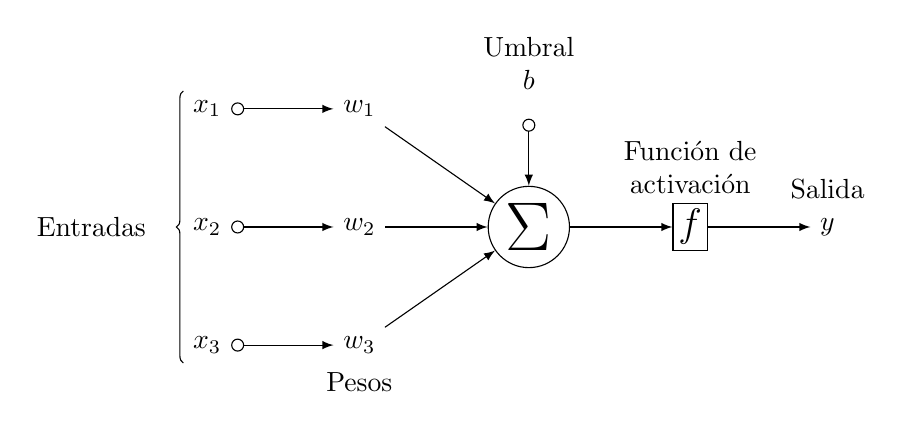
\begin{tikzpicture}[
init/.style={
  draw,
  circle,
  inner sep=2pt,
  font=\Huge,
  join = by -latex
},
squa/.style={
  draw,
  inner sep=2pt,
  font=\Large,
  join = by -latex
},
start chain=2,node distance=13mm
]
\node[on chain=2] 
  (x2) {$x_2$};
\node[on chain=2,join=by o-latex] 
  {$w_2$};
\node[on chain=2,init] (sigma) 
  {$\displaystyle\Sigma$};
\node[on chain=2,squa,label=above:{\parbox{2cm}{\centering Función de\\ activación }}]   
  {$f$};
\node[on chain=2,label=above:Salida,join=by -latex] 
  {$y$};
  
\begin{scope}[start chain=1]

\node[on chain=1] at (0,1.5cm) 
  (x1) {$x_1$};
\node[on chain=1,join=by o-latex] 
  (w1) {$w_1$};
  
\end{scope}
\begin{scope}[start chain=3]
\node[on chain=3] at (0,-1.5cm) 
  (x3) {$x_3$};
\node[on chain=3,label=below:Pesos,join=by o-latex] 
  (w3) {$w_3$};
\end{scope}

\node[label=above:\parbox{2cm}{\centering Umbral \\ $b$}] at (sigma|-w1) (wo) {};

\draw[-latex] (w1) -- (sigma);
\draw[-latex] (w3) -- (sigma);
\draw[o-latex] (wo) -- (sigma);

\draw[decorate,decoration={brace,mirror}] (x1.north west) -- node[left=10pt] {Entradas} (x3.south west);

\end{tikzpicture}
}
\centering
\caption{Representacion de una Red Neuronal Artificial.}
\label{fig:RNA}
\end{figure}

\begin{enumerate}
  \item Las \textbf{entradas} $x_i$, que son puntos por los que se reciben los datos provenientes del entorno o bien de otras neuronas. Para este caso se consideran $n$ entradas, siendo el valor de $n=3$
  \[ X = (x_1,x_2,x_3)\]
  
  \item La salida $y_i$. En una neurona biológica corresponde al axón
  \item Al igual que en una neurona biológica, la neurona artificial debe permitir establecer conexiones(sinápsis) entre las entradas(dendritas) de una neurona y la salida (axón) de otra. Esta conexión representa con una línea que tiene asociado un valor llamado \textbf{peso sináptico} $w_ji$. Nótese que el primer subíndice indice la neurona a la que llega la conexión, mientras que el segundo subíndice indica de donde viene la conexión. El peso representa el factor de importancia de la conexión en la determinación del valor de salida. El valor $w_ji$, que es un número real, se modifica durante el entrenamiento de la red neuronal y es la variable de almacenará la información que indicará que la red ha aprendido algo y por tanto que sirva para un propósito u otro.
  
  \item En la Figura \ref{fig:RNA} también se observa una entrada especial, llamada umbral, con un valor fijo que puede ser -1 o 1, y con un peso asociado llamado $w_0$. El valor del umbral se ajusta igual que cualquier otro peso durante el proceso de entrenamiento.
  
  \item Una \textbf{regla de propagación}. Para cierto valor de las entradas $x_i$ y los pesos sinápticos asociados $w_ji$, se realiza algun tipo de operación para obtener el valor del potencial \textit{post-sináptico} . Este valor es función de las entradas y los pesos. Una de las operaciones mas comunes es realizar la suma ponderada, que no es otra cosa que la sumatoria de las entradas, pero teniendo en cuenta la importancia de cada una (el peso sináptico asociado). Luego:


\[u=\sum_{i}^{\ n=3} w_{ji}x_i + w_0b\]


\item Una \textbf{función de activación}. Luego de realizar la suma ponderada, se aplica al resultado la función de activación, que se escoge de tal manera que permita obtener la forma deseada para el valor de la salida.

\begin{equation} \label{eq1}
\begin{split}
y 	&= f(u)\\
	&= f(\sum_{i}^{\ n=3} w_{ji}x_i + w_0b)\\
	&= f(W.X)\\
	&= f(W^TX)
\end{split}
\end{equation}

donde las últimas dos ecuaciones están en notación vectorial.
Es necesario especificar la función de activación $f$. Las funciones más usuales se observan en la  \ref{fig:FUNCACT}

Con estas especificaciones, se puede ahora explicar cómo funciona la neurona. Se supone en el modelo de neurona más simple, que corresponde a la función de activación escalón, tambien llamada limitador duro. En este caso, la salida puede tomar solo dos valores -1 y +1 donde la salida esta determinada por

\begin{equation}\label{eq2}
f(x) = \begin{cases}
             -1  & \text{if } u < 0 \\
             +1  & \text{if } u \ge 0
       \end{cases} \quad
\end{equation}

\clearpage

\begin{figure}[h]
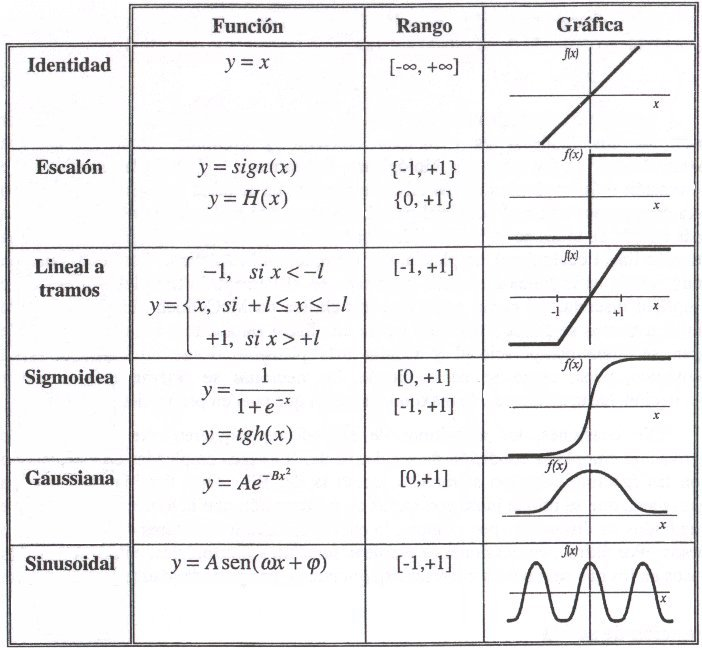
\includegraphics[width=\textwidth]{list_function}
\centering
\caption{Funciones de activación.}
\label{fig:FUNCACT}
\end{figure}

Entonces, para la función sigmoidea, se tiene que

\begin{equation} \label{eq3}
\begin{split}
y 	&= ( \frac{1}{1+e^{-u}}) \\
u	&= \sum_{i}^{\ n=3} w_{ji}x_i + w_0b
\end{split}
\end{equation}

y para el segundo caso de la función sigmoidea

\begin{equation} \label{eq3}
\begin{split}
y 	&= tanh(u) = ( \frac{e^u - e^{-u}}{e^u + e^{-u}}) \\
\end{split}
\end{equation}

La expresión de la ecuación que almacena la neurona en virtud del vector de pesos $W$ es el \textbf{modelo} que representa en mayor o menor grado el comportamiento del vector de salida y con respecto al vector de entrada $X$

\end{enumerate}

Entonces, una neurona artificial es un procesador elemental. Se encarga de procesar un vector de $n$ entradas para producir un único valor de salida $y$. El nivel de activación depende de las entradas recibidas y de los valores sinápticos. Para calcular el estado de activación se ha de calcular en primer lugar la entrada total a la célula. Este valor se cálcula como la suma de todas las entradas ponderadas por ciertos valores dados a la entrada.

\clearpage

\subsection{Redes Neuronales Artificiales}
La capacidad de modelar funciones más complejas aumenta grandemente cuando la neurona no trabaja sola, sino interconectada con otras neuronas, formando Redes Neuronales Artificiales (RNA), tal como se observa de manera simplificada en la Figura \ref{fig:MLP}


\begin{figure}[h]
\frame{
\tikzset{%
  every neuron/.style={
    circle,
    draw,
    minimum size=1cm
  },
  neuron missing/.style={
    draw=none, 
    scale=4,
    text height=0.333cm,
    execute at begin node=\color{black}$\vdots$
  },
}

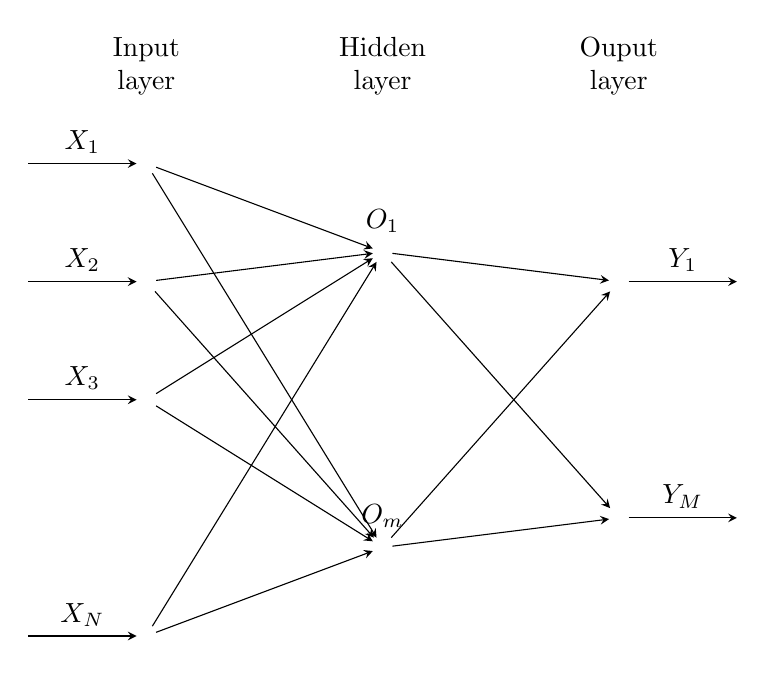
\begin{tikzpicture}[x=1.5cm, y=1.5cm, >=stealth]

\foreach \m/\l [count=\y] in {1,2,3,missing,4}
  \node [every neuron/.try, neuron \m/.try] (input-\m) at (0,2.5-\y) {};

\foreach \m [count=\y] in {1,missing,2}
  \node [every neuron/.try, neuron \m/.try ] (hidden-\m) at (2,2-\y*1.25) {};

\foreach \m [count=\y] in {1,missing,2}
  \node [every neuron/.try, neuron \m/.try ] (output-\m) at (4,1.5-\y) {};

\foreach \l [count=\i] in {1,2,3,N}
  \draw [<-] (input-\i) -- ++(-1,0)
    node [above, midway] {$X_\l$};

\foreach \l [count=\i] in {1,m}
  \node [above] at (hidden-\i.north) {$O_\l$};

\foreach \l [count=\i] in {1,M}
  \draw [->] (output-\i) -- ++(1,0)
    node [above, midway] {$Y_\l$};

\foreach \i in {1,...,4}
  \foreach \j in {1,...,2}
    \draw [->] (input-\i) -- (hidden-\j);

\foreach \i in {1,...,2}
  \foreach \j in {1,...,2}
    \draw [->] (hidden-\i) -- (output-\j);

\foreach \l [count=\x from 0] in {Input, Hidden, Ouput}
  \node [align=center, above] at (\x*2,2) {\l \\ layer};

\end{tikzpicture}

}
\centering
\caption{Topologia de la Red Perceptron Multicapa.}
\label{fig:MLP}
\end{figure}


La red mas simple se llama \textbf{perceptron multicapa}. Esta red define una relación entre las variables de entrada y las variables de salida. Esta relación se obtiene \textit{propagando} hacia adelante los valoers de las variables de entrada. Cada neurona procesa las información recibida por sus entradas y produce una respuesta o activación que se propaga, a través de las conexiones correspondientes, hacia las neuronas de la siguiente capa.\hfill \break

Sea un perceptron multicapa con $C$ capas, de las cuales una es la capa de entrada, una la capa de salida y $C-2$ capas ocultas. Se tiene $n_c$ neuronas en la capa $c$, con $c= 1,2,3,....,C$. sea $W^c = (w_{ji}^c)$ la matriz de pesos asociada a las conexiones de la capa $c$ a la capa $c+1$ para $c=1,2,3,...,C-1$, donde $w_{ji}^c$ representa el peso de la conexión de la neurona $i$ de la capa $C$ a la neurona $j$ de la capa $C+1$. Sea $U^c = (u_j^c)$ el vector de umbrales  de las neuronas de la capa $c$ para $c=2,3,...,C$. Se denota $o_j^c$ a la activación de la neurona $j$ de la capa $c$; estas activaciones se calculan del siguiente modo:



\begin{enumerate}
\item 
Entrada $(o_i^1)$. Estas neuronas transmiten hacia la red las señales recibidas del exterior

\begin{equation} \label{eq4}
o_j^1 = x_j \quad para \quad j=1,2,3,...n_1
\end{equation}

Donde  $X = (x_1,x_2,...,x_n)$ representan el vector de entrada a la red.

\item
Activación de las neuronas de  la capa oculta $c (o_j^c)$: Las neuronas ocutas procesan la informacion recibida aplicando la función de activación $f$ a la suma de los productos de las activaciones que recibe por sus correspondientes pesos:


\begin{equation} \label{eq5}
o_j^c = f(\sum_{i=1}^{\ n_{c-1}} w_{ji}^{c-1}o_i^{c-1} + u_j^c)
\end{equation}

Para $j = 1,2,3,....,n_c \quad y \quad c=2,3,...,c-1$

\item
Salida $(a_i^C)$ : Al igual que en las capas ocultas, la activación de estas neuronas viene dada por la función de activación $f$

\begin{equation} \label{eq6}
y_j = o_j^c = f(\sum_{i=1}^{\ n_{c-1}} w_{ji}^{c-1}o_i^{c-1} + u_j^c)
\end{equation}

Para $j=1,2,3,...,n_c \quad donde \quad Y=(y_1,y_2,,y_3,...,y_c)$ es el vector de salida de la red.

\end{enumerate}

Para el perecptron multicapa las funciones de activación mas usadas son la funciones \textbf{sigmoidal}:

\begin{equation} \label{eq7}
f(u) = \frac{1}{1+e^{-u}})
\end{equation}

y la función \textbf{tangente hiperbólica}

\begin{equation} \label{eq8}
f(u) = ( \frac{1 - e^{-u}}{1 + e^{-u}}) 
\end{equation}

Estas funciones tienen una forma similar pero se diferencian en que la sigmoidal tiene un rango continuo de valores dentro de los intervalor $[0,1]$ mientras que la tangente hiperbólica tiene un rango contínuo en el intervalo $[-1,1]$.


\section{Caso de Estudio}
Todos los días, millones de e-mails invaden las bandejas de entrada de los usuarios de Internet. De todos éstos, una cantidad muy importante es considerada "correo basura". Compuesto por mensajes publicitarios no solicitados, cadenas de la suerte o incluso virus que se autoenvían, el spam afecta a más de un usuario, y
hace que la tarea de revisar el correo sea una verdadera molestia.
El problema fundamental lo representan los spams, que son mensajes publicitarios no solicitados. Ya no resulta raro para quienes contamos con una
dirección de correo electrónico recibir a diario varios mensajes con propagandas de las más variadas temáticas. A pesar de que ningún método de detección de Spam es totalmente efectivo, consideramos que si es posible mejorar los existentes y reducir considerablemente las deficiencias que actualmente presentan las herramientas disponibles. Es un hecho que parte de los mensajes no deseados escapan a los sistemas de detección de correo basura constituyendo así un "falso negativo", igualmente existe la posibilidad de identificar un mensaje como Spam sin serlo, lo que se conoce como "falso positivo". La idea es tomar las máximas precauciones posibles para minimizar este efecto, y para ello se debe ser consciente de este hecho antes de adoptar las posibles medidas de filtrado que se propondrá.\cite{emailspam}
\subsection{Problema}
El crecimiento de Internet a nivel mundial esta cambiando nuestra forma de comunicación entre otros, por lo que cada vez la gente utiliza más el correo electrónico. A causa de un número tentativo de correos electrónicos los publicistas y spammers se ven los modos para obtener un listado grande de correos y así poder enviar spam. Todos los días, billones de e-mails invaden las bandejas de entrada de los usuarios de Internet. De todos éstos, una cantidad muy importante es considerada "correo basura". Compuesto por mensajes publicitarios no solicitados, cadenas de la suerte o incluso virus que se auto envían, el spam aqueja a más de un usuario, y hace que la tarea de revisar correo sea una verdadera molestia.\cite{emailspam}

Los principales problemas son los siguientes:
\begin{itemize}
\item Perdida de productividad y dinero en las empresas
\item Amenaza la viabilidad de Internet como un medio efectivo de comunicación.
\item Incremento de costos relacionados con el tiempo.
\item Genera importantes costos de seguridad a empresas ISP’s.
\item Incremento de propagación de virus informáticos.
\item Saturación de servidores. Muchos servidores
dedicados para uso privado o para uso general son
congestionados implicando una reducción decalidad
de servicio.
\item Denegación de servicios (Deny of services). Una
cantidad excesiva de correos no deseados puedo
congestionar totalmente el servicio y así denegarlo al
mismo.
\item Buzón de entrada incontrolable por parte del
receptor. Causado por la cantidad masiva que los
spammers envían a los correos electrónicos.
\item Daño de imagen a terceros.
\item Molestias por parte del receptor.
\end{itemize}

\subsection{Justificacion}
El correo electrónico, es sin duda un medio
que nos permite comunicar rápidamente ofreciéndonos reducción de tiempo y costo Sin
embargo muchas personas aprovechan esto para
utilizarlo de forma no legítima con fines publicitarios,
ocasionando una serie de problemas a
nivel personal comoempresarial.
Como contramedida a esta acción se
necesitan herramientass capaces de reducir el spam.
De esta manera es muy importante la
elaboración de anti-spams, ya que es la forma más
viable de acabar con el spam y ofrecer a los
usuarios seguridad y tranquilidad en los correos
electrónicos, y por otra parte reducir los costos para
las empresas ISP’s y controlar la saturación
de servidores de correo electrónico.
\textbf{El desarrollo de una
herramienta informática capaz de aminorar con los
problemas que causa el spam}, no es solamente capaz
de \textbf{ahorrar mucho dinero} en aquellas empresas que
suelen estar perjudicadas con el spam, sino también es
capaz de permitir una mejor utilización y minimizar
los dolores de cabeza a cualquier usuario del correo
electrónico.\cite{emailspam}
\subsection{Propuestas de Red Neuronal}
Las redes neuronales tienen un gran poder en los algoritmos de Machine Learning. Ellos puedes ser usados para transformar las caracteristicas como un forma bastante compleja de decisión no lineal. Dentro de estos se encuentras el percetron multicapa que en primera instancia se puede utilizar para problemas de clasificación.

Como el problema que estamos tratando en este documento es un problema comun de clasificación donde la red neuronal debera clasificar si un determinado email es o no es spam. En este problema, nosotros estamos dando un paquete de correos(que ya estan normalizados.) and la red neuronal decidirá si cada email es o no es spam. Depues de determinar los pesos fijos de la red le presentaremos  un nueva conjunto de correos (test data) y evaluaremos si estos correos son o no  correos spam.
\subsubsection{Topologia}
Tenemos tres capas en la red neuronal para la detección de spam.
\begin{itemize}
\item La primera capa son los datos de entrada que tienen 57 neuronas, 1 neurona por cada caracteristica del correo.

\item La segunda capa es la capa intermedia que tiene 4 neuronas

\item La capa final o de salida tiene 1 sola neurona que indica si es o no es spam
\end{itemize}
\clearpage

\begin{figure}[h]
\frame{
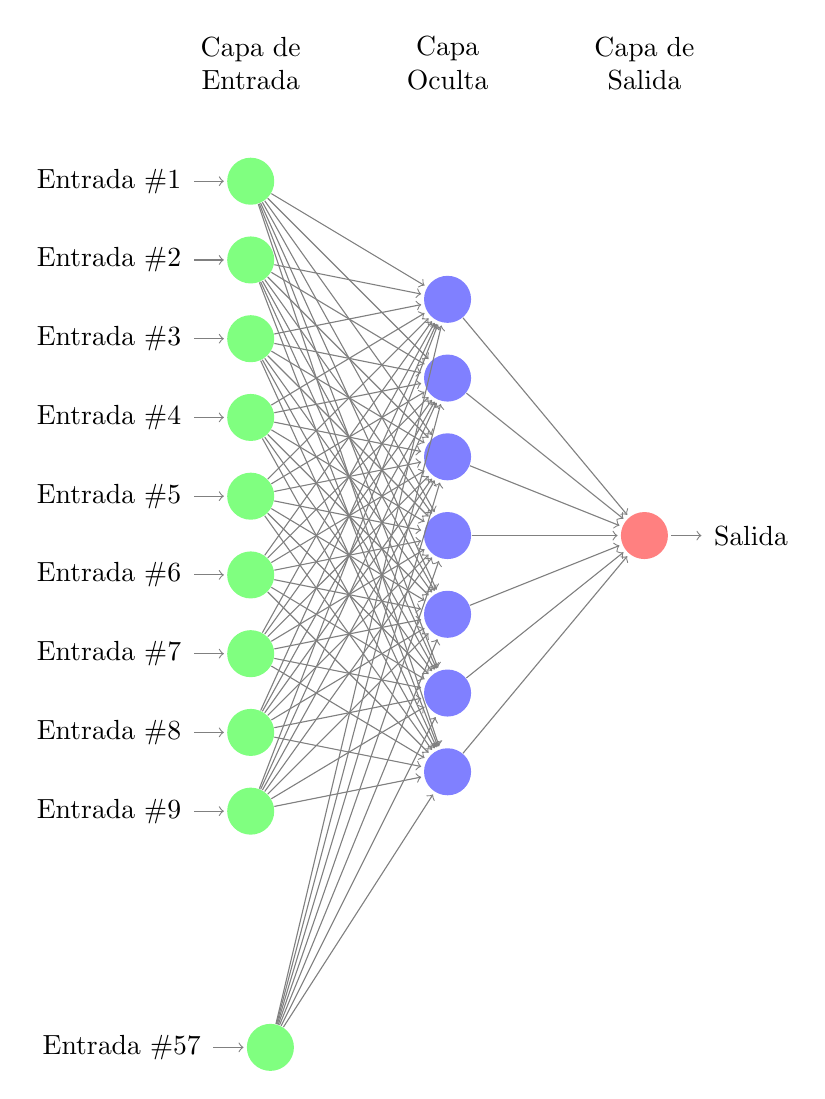
\begin{tikzpicture}[shorten >=1pt,->,draw=black!50, node distance=\layersep]
    \tikzstyle{every pin edge}=[<-,shorten <=1pt]
    \tikzstyle{neuron}=[circle,fill=black!25,minimum size=17pt,inner sep=0pt]
    \tikzstyle{input neuron}=[neuron, fill=green!50];
    \tikzstyle{output neuron}=[neuron, fill=red!50];
    \tikzstyle{hidden neuron}=[neuron, fill=blue!50];
    \tikzstyle{annot} = [text width=4em, text centered]


    \foreach \name / \y in {1,...,9}
        \node[input neuron, pin=left:Entrada \#\y ] (I-\name) at (0,-\y) {};
     
     \node[input neuron, pin=left:Entrada \#57] (I-10) at (.25,-12) {};


    \foreach \name / \y in {1,...,7}
        \path[yshift=-1.5cm]
            node[hidden neuron] (H-\name) at (\layersep,-\y cm) {};

    % Draw the output layer node
    \node[output neuron,pin={[pin edge={->}]right:Salida}, right of=H-4] (O) {};

    % Connect every node in the input layer with every node in the
    % hidden layer.
    \foreach \source in {1,...,9}
        \foreach \dest in {1,...,7}
            \path (I-\source) edge (H-\dest);
     
    \path (I-10) edge (H-1);
    \path (I-10) edge (H-2);
    \path (I-10) edge (H-3);
    \path (I-10) edge (H-4);
    \path (I-10) edge (H-5);
    \path (I-10) edge (H-6);
    \path (I-10) edge (H-7);

    % Connect every node in the hidden layer with the output layer
    \foreach \source in {1,...,7}
        \path (H-\source) edge (O);

    % Annotate the layers
    \node[annot,above of=H-1, node distance=3cm] (hl) {Capa Oculta};
    \node[annot,left of=hl] {Capa de Entrada};
    \node[annot,right of=hl] {Capa de Salida};
\end{tikzpicture}
}
\centering
\caption{Topologia de la Red Perceptron Multicapa para la detección de correos spam.}
\label{fig:MLP}
\end{figure}

\subsubsection{Reglas}

\subsubsubsection{Regla de propagación}
La regla de propagación esta determinada por la sumatoria de las entradas y los pesos, tomando como otra entrada a la neurona el $bias$.

\begin{equation}
u_j^c = \sum_{i=0}^{\ n_{c-1}} w_{ji}^{c-1}x_i^{c-1}
\end{equation}

\subsubsubsection{Regla de Activacion}
La funcion de activación esta determinada por la funcion sigmoide.

\begin{equation} \label{eq3}
\begin{split}
y 	&= ( \frac{1}{1+e^{-u_j^c}}) \\
u	&= \sum_{i=0}^{\ n} w_{ji}x_i
\end{split}
\end{equation}

Entonces la salida con esta función, tiene la siguiente forma

\begin{equation} \label{eq1}
\begin{split}
y 	&= f(u)\\
	&= f(\sum_{i=0}^{\ n} w_{ji}x_i)\\
	&= ( \frac{1}{1+e^{-\sum_{i=0}^{\ n} w_{ji}x_i}}) \\
\end{split}
\end{equation}


\subsubsubsection{Regla de Salida}
Finalmente la regla de salida esta determinada por
\begin{equation} \label{eq1}
\begin{split}
y_j^c 	&= f(u_j^c)\\
		&= f(\sum_{i=0}^{\ n_{c-1}} w_{ji}^{c-1}x_i^{c-1})\\
		&=  \frac{1}{1+e^{-\sum_{i=0}^{\ n_{c-1}} w_{ji}^{c-1}x_i^{c-1}}} \\
\end{split}
\end{equation}
\subsubsubsection{Regla de Aprendizaje}
Se han planteado tres reglas de aprendizaje, cada una de estas seran descritas a continuación.
\subsubsubsubsection{Back Propagation}
Es la regla mas comun, para poder exlicar la regla de aprendizaje mediante propagación hacia atras, se tomara como ejemplo la la arquitectura planteada en\ref{fig:MLP}

Considerando que tenemos dos capas, dado que la capa de entrada no hace ninguna operación, entonces:

\begin{itemize}
\item Capa I
\begin{equation} \label{eq9}
\begin{split}
v_j^I = <w_j^I, X> = \sum_{i=0}^{\ N} w_{ji}^I x_i \\
y_j^I =  f(v_j^I) = \frac{1}{1 + e^{-v_j^I}}
\end{split}
\end{equation}

\item Capa II
\begin{equation} \label{eq10}
v_j^II = <w_j^II, y^I> 
y_j^II =  f(v_j^II) 
\end{equation}
\end{itemize}

Ahora para cada salida que tengamos de la capa II, calculamos el error total cometido, de la siguiente manera:

\begin{equation} \label{eq11}
\xi (n) = \frac{1}{2} \sum_{j=1}{M}e_j^2(n)
\end{equation}
Elevar al cuadro tiene mucha importancia dado que, imaginemos que en una salida $y_x$ el error sea $-1$ y en otra salida $y_k$ el error sea $-1$ al sumarlo el error total resultaría cero, entonces, al elevarlo al cuadrado tiene agunas ventajas como la mencionada.

La regla de progapación hacia atras consiste en modificar los pesos para lograr el menor error posible,  para lograr esto debemos recordar la utilidad que tiene  el gradiente de una función:

\textit{La gradiente  o también conocido  como vector gradiente, es un campo vectorial.El vector gradiente  de una funcion $f$ evaluado en un punto generico $x$ del  dominino de $f$, indica la dirección en la cual  el campo $f$ varía mas rápidamente y su módulo representa el ritmo de variación  de $f$ en la dirección de dicho vector gradiente.}\cite{gradient}

\clearpage

\begin{figure}[h]
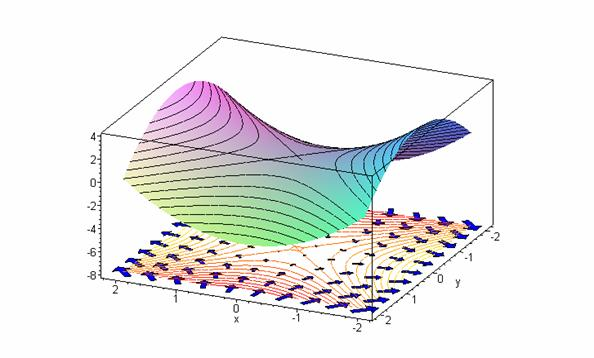
\includegraphics[width=\textwidth]{gradiente}
\centering
\caption{Gradiente de una función $f$.}
\label{fig:GRADIENT}
\end{figure}

Entonces para lograr disminuir el error, aplicaremos la siguiente variación:

\begin{equation} \label{eq11}
\nabla w_{ji}(n) =  -\mu \frac{\partial \xi(n)}{\partial w_{ji}(n)}
\end{equation}

\subsubsubsubsection{Metodo de Segundo Orden (Levenger - Marquardt)}

El método de Levenger - Marquardt es un tipo de algoritmo de entrenamiento similar a los denominados quasi-Newton. Para entender la funcionalidad del método LM es conveniente empezar por comprender el método de Newton. El método
de Newton es un método de segundo orden que constituye una alternativa a los métodos de gradiente conjugado para optimización rápida. El paso básico del método de Newton
durante la época n es

\begin{equation}
w(n+1) = w(n) - H(n)^{-1}g(n)
\end{equation}

donde $w$ es el vector de pesos, $g(n)$ es el vector gradiente actual y $H(n)$ es la matriz Hessiana (de derivadas segundas) de la función de error respecto a los pesos, evaluada en los valores actuales de pesos y umbrales. El método de Newton generalmente converge más rápido que los métodos de gradiente conjugado. Desafortunadamente, la matriz Hessiana es compleja y costosa de calcular para las redes feedforward. Los algoritmos
denominados quasi-Newton (método de la secante) calculan y actualizan una aproximación de la matriz Hessiana sin necesidad de resolver las derivadas de segundo orden en cada iteración. La actualización realizada es función del gradiente.
Al igual que los métodos quasi-Newton, el algoritmo LM fue diseñado para acometer entrenamientos rápidos de segundo orden sin tener que calcular la matriz Hessiana.
Cuando la función de error tiene la forma de una suma de cuadrados (el caso típico en las redes feedforward ), entonces la matriz Hessiana puede aproximarse como

\begin{equation}
H = J^TJ
\end{equation}

donde $J$ es la matriz Jacobiana que contiene las primeras derivadas de la función de error de la red respecto a los pesos y umbrales. El gradiente se obtiene como

\begin{equation}
g=J^Te
\end{equation}

siendo e el vector de errores de la red. El cálculo de la matriz Jacobiana se reduce a un simple cálculo del algoritmo de retropropagación que es mucho más sencillo que
construir la matriz Hessiana. El método LM actualiza los pesos de forma similar al método de Newton pero introduciendo los cambios anteriores:

\begin{equation}
w(n+1) = w(n)[\textbf{J}^TJ + \mu I]^1\textbf{J}^Te
\end{equation}

donde el parámetro $\mu$ actua como tasa de aprendizaje. Cuando $\mu$ es cero, el algoritmo
se convierte en el método de Newton empleando la forma aproximada del cálculo de la matriz Hessiana:

\begin{equation}
w(n+1) = w(n)H^1g
\end{equation}

Cuando $\mu$ es grande, se puede despreciar la aportación de la matriz Hessiana al cálculo y obtenemos el método de descenso de gradiente con un tamaño de paso $(\frac{1}{\mu}):$

\begin{equation}
w(n+1) = w(n)\frac{1}{u}g
\end{equation}

El método de Newton es más eficaz cerca de un mínimo de error, así que el objetivo es migrar al método de Newton tan pronto como sea posible. Así pues, se reduce $\mu$ tras cada paso exitoso (cada vez que el error se logra reducir) y solo se aumenta cuando el
error aumenta respecto a la iteración anterior. Con esta metodología, la función de error siempre disminuye tras cada iteración del algoritmo.
El algoritmo LM parece ser el método más rápido para entrenar redes feedforward de tamaño moderado (hasta varios centenares de parámetros). Su principal desventaja es que requiere almacenar las matrices Jacobianas que, para ciertos conjuntos de datos,
pueden ser muy grandes, lo que significa un gran uso de memoria.

\subsubsubsubsection{R-PROP}
El algoritmo RPROP cálcula el cambio de los pesos en forma separada, es guiado por laprimera derivada de $f$ , en este caso; $f$ es una medida de la diferencia entre la salida arrojada por la red neuronal y el valor esperado. RPROP utiliza parámetros independientes que controlan la velocidad con que se recorre la función objetivo para cada uno de los pesos de la red neuronal, al no verse afectado por la saturación de la red neuronal converge mas rápidamente que otros algoritmos

Un perceptron multicapa busca  una función $y_t$ que se construye  en funcion  de sus valores  pasados, $y_{y-1}, y_{t-2}, ...., y_{t-P}$.

\begin{equation}
y_t = \beta_* + \sum_{H}^{h=1}\beta_hg [\frac{1}{2\sigma_y^-1}(\alpha_{x,j} + \sum_{p=1}^{P}\alpha_{p,h}y_{t-p})] + \xi_t
\end{equation}

Donde los parametros $\omega = [\beta_*, \beta_h, \alpha_{*,h}, \alpha_{p,h}], h=1...H, p=1...P$ son estimados usando el principio de máxima versomilitud de los residuales, el cual equivale a la minimización de una función de costo que es definida usualmente como error cuadratico medio. Esta ecuación equivale a un modelo estadístico no paramétrico de regresión no lineal, $\xi_t$ sigue una distribución normal con media cero y varianza desconocida $\sigma^2$; $H$ representa el númerode neuronas en la capa oculta,$P$ es el número de rezagos de la variable dependiente y $g$ es la función de activación de las neuronas de la capa oculta.

El algoritmo RPROP busca encontrar los valores del vector de parámetros $\omega$, de forma que se minimice la diferencia entre los valores reales $y_t^*$ y los valores de $y_t$.

La actualización de los pesos, viene dada por

\begin{equation}
\triangle w_{ji}(n) = -\alpha(n) signo(\nabla_{w_{j,i}(n)}E)
\end{equation}

La utilizacion del signo del gradiente en la actualización de los pesos supone un ahorro en la carga computacional. Por otro lado, la constante  de adaptación viene dada por
\begin{equation}
\alpha(n) = 
\begin{cases}
\alpha(n) = 	min(	\alpha(n)u,\alpha_{max}) \longleftrightarrow (\nabla_{w_{j,i}(n)}E)(\nabla_{w_{j,i}(n-1)}E)>0 \\
max(	\alpha(n)d,\alpha_{min}) \longleftrightarrow (\nabla_{w_{j,i}(n)}E)(\nabla_{w_{j,i}(n-1)}E)>0 \\
\end{cases} \quad
\end{equation}

con $u > 1$ y $ d < 1 $.

Se intenta tener un valor bajo en las proximidades del mínimo y mayor lejos de éste.controlando de esta manera la velocidad de convergencia, pero se limitan los valores ya quesi son demasiado grandes se pueden tener inestabilidades y si son demasiado pequeños lavelocidad de convergencia puede ser muy lenta.

\subsection{Desarrollo de la solucion}
Para el desarrollo del perceptrón multicapa planteado anteriormente hemos se escogio como primera herramienta $R$( Figura \ref{Fig:R}) y con el IDE Rstudio( Figura \ref{Fig:RSTUDIO}), pero no se utilizo  porque \textbf{el tiempo de aprendizaje para un numero mayor de 10 epocas era muy elevado}, a comparacion de la segunda herramienta, python.

\clearpage

\begin{figure}[!htb]
   \begin{minipage}{0.48\textwidth}
     \centering
     
\includegraphics[width=.7\linewidth]{rstudio}
     \caption{IDE Rstudio}
     \label{Fig:RSTUDIO}
   \end{minipage}\hfill
   \begin {minipage}{0.48\textwidth}
     \centering
     
\includegraphics[width=.7\linewidth]{r}
     \caption{Lenguaje R}
     \label{Fig:R}
   \end{minipage}
\end{figure}

\subsubsection{Herramientas}
Como se dijo anteriormente no se utilizó la herramienta R debido a su alto tiempo en procesar la información, a continuación se describen las herramientas utilizadas.

\subsubsubsection{Python}
Python es un lenguaje de programación interpretado cuya filosofía hace hincapié en una sintaxis que favorezca un código legible.

Se trata de un lenguaje de programación multiparadigma, ya que soporta orientación a objetos, programación imperativa y, en menor medida, programación funcional. Es un lenguaje interpretado, usa tipado dinámico y es multiplataforma.

Es administrado por la Python Software Foundation. Posee una licencia de código abierto, denominada Python Software Foundation License,1 que es compatible con la Licencia pública general de GNU a partir de la versión 2.1.1, e incompatible en ciertas versiones anteriores.\cite{python}

\begin{figure}[h]

\includegraphics[width=3cm, height=3cm]{python}
\centering
\caption{Lenguaje Python.}
\label{fig:FUNCACT}
\end{figure}

\subsubsubsection{PyCharm}
El entorno de desarrollo integrado que se utilizo es PyCharm, es un entorno muy popular utilizado en la comunidad de python que provee una manera sencilla de programar en python eligiendo la version de python que deseamos compilar y agregar los packetes necesarios para el desarrollo de nuestros proyectos.

\begin{figure}[h]

\includegraphics[width=3cm, height=3cm]{pycharm}
\centering
\caption{IDE Pycharm.}
\label{fig:FUNCACT}
\end{figure}

\subsubsubsection{Package}
Para el desarrollo de los algoritmos de aprendizaje para el perceptron multicapa se utilizo una libreria para Inteligencia Artificial llamada NeuPy. Esta libreria actualmente en su version 0.6 soporta diferentes tipos de Redes Neuronales desde un perceptron simple hasta modelos de deep learning \cite{neupy}.

Actualmente soporta la siguientes características:

\begin{itemize}
\item Deep Learning
\item Reinforcement Learning (RL)
\item Convolutional Neuronal Networks (CNN)
\item Recurrent Neuronal Networks (RNN)
\item Restricted Boltzmann Machine (RBM)
\item Multilayer Perceptron (MLP)
\item Networks based on the Radial Basis Functions (RBFN)
\item Ensemble Networks
\item Competitive Networks
\item Basic Linear Networks
\item Regularizartion Algorithms
\item Step Update Algorithms
\end{itemize}

\begin{figure}[h]

\includegraphics[width=3.5cm, height=3.5cm]{neupy}
\centering
\caption{Funciones de activación.}
\label{fig:FUNCACT}
\end{figure}

\subsubsection{Implementacion}
A continuación pasaremos a describir los métodos de aprendizaje para nuestro perceptron multicapa.
\subsubsubsection{Back Propagation}

Para describir mejor el procedimientos pasaremos de describir el codigo por partes:
\begin{enumerate}
\item
Se procede a importar los paquetes necesarios para la implementación, creamos las funciones de activación y la funcion derivada
\newline
\begin{figure}[h]
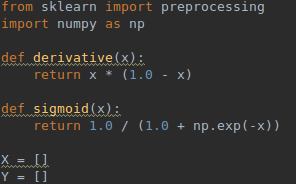
\includegraphics[width=5cm, height=2cm]{mlp_import}
\centering
\caption{Importar paquetes necesarios.}
\label{fig:RPROP_IMPORT}
\end{figure}

\item
Ahora leeremos nuestro archivo $Train.csv$ que contiene los datos normalizados
 \begin{figure}[h]
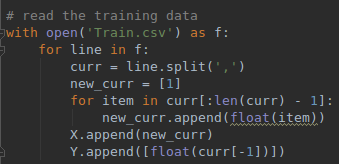
\includegraphics[width=6cm, height=2cm]{mlp_read}
\centering
\caption{Leer la data de entrenamiento.}
\label{fig:RPROP_INIT}
\end{figure}

\item
Asignamos los valores a nuestros arreglos para poder guardar los valores locales que se van creando, al igual que los valores random para los pesos iniciales
 \begin{figure}[h]
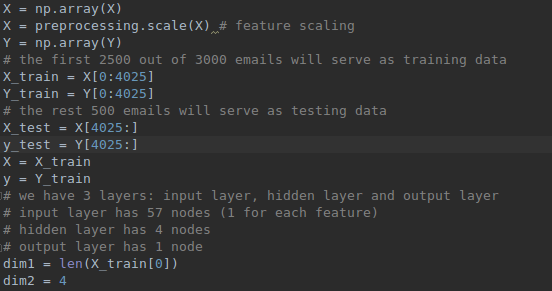
\includegraphics[width=8cm, height=3cm]{mlp_assign}
\centering
\caption{Asignar valores de entrada a nuestros arreglos.}
\label{fig:RPROP_READ}
\end{figure}

\item
Llamamos al metodo de Rprop de la liberia neuPy para poder pasarle los parametros de entrada y las configuraciones necesarias
\begin{figure}[h]
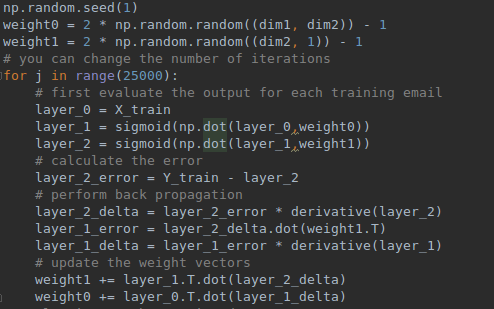
\includegraphics[width=8cm, height=3cm]{mlp_train}
\centering
\caption{Crear las epocas y comenzar a iterar.}
\label{fig:RPROP_READ}
\end{figure}

\clearpage
\item
Finalmente Podemos mostrar los valores que se han obtenido luego del entrenamiento y del recuerdo
 \begin{figure}[h]
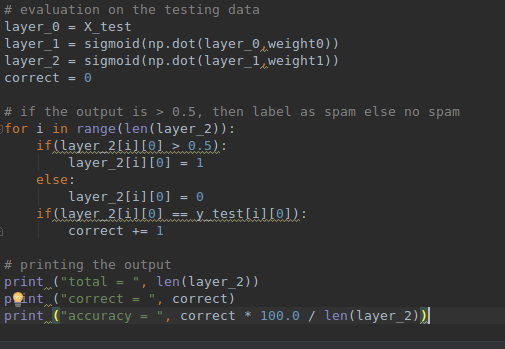
\includegraphics[width=8cm, height=3cm]{mlp_result}	
\centering
\caption{Imprimir los resultados.}
\label{fig:RPROP_READ}
\end{figure}

\end{enumerate}


\subsubsubsection{R-PROP}
Para describir mejor el procedimientos pasaremos de describir el codigo por partes:
\begin{enumerate}
\item
Se procede a importar los paquetes necesarios para la implementación
\newline
\begin{figure}[h]
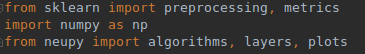
\includegraphics[width=6cm, height=2cm]{rprop_import}
\centering
\caption{Importar paquetes necesarios.}
\label{fig:RPROP_IMPORT}
\end{figure}

\item
 Ahora asignaremos nuestros vectores de entrada y salida respectivamente.
 \begin{figure}[h]
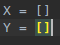
\includegraphics[width=3cm, height=1.5cm]{rprop_init}
\centering
\caption{Inicializar vectores.}
\label{fig:RPROP_INIT}
\end{figure}
\clearpage
\item
Se procede a leer la data de entrenamiento
 \begin{figure}[h]
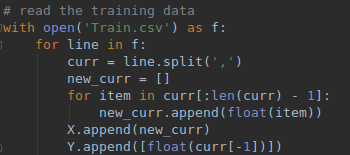
\includegraphics[width=8cm, height=3cm]{rprop_read}
\centering
\caption{Leer data de entrenamiento.}
\label{fig:RPROP_READ}
\end{figure}

\item
Asignamos los valores a nuestros arreglos para poder guardar los valores locales que se van creando
 \begin{figure}[h]
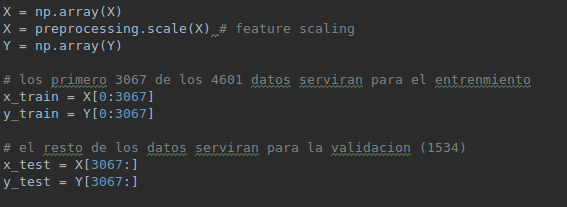
\includegraphics[width=8cm, height=3cm]{rprop_assign}
\centering
\caption{Asignar valores de entrada a nuestros arreglos.}
\label{fig:RPROP_READ}
\end{figure}

\item
Llamamos al metodo de Rprop de la liberia neuPy para poder pasarle los parametros de entrada y las configuraciones necesarias
\begin{figure}[h]
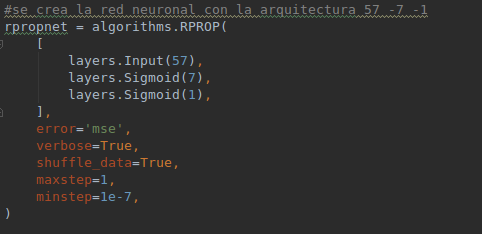
\includegraphics[width=8cm, height=3cm]{rprop_creation}
\centering
\caption{Llamar al constructor del RPROP.}
\label{fig:RPROP_READ}
\end{figure}

\clearpage
\item
Finalmente Podemos mostrar los valores que se han obtenido luego del entrenamiento y del recuerdo
 \begin{figure}[h]
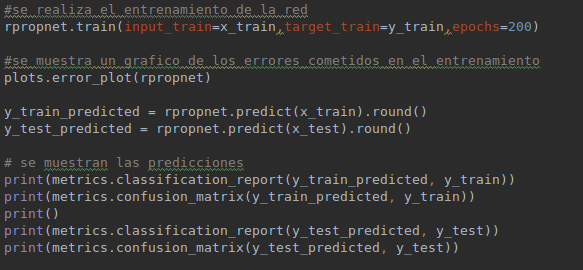
\includegraphics[width=8cm, height=3cm]{rprop_finalize}
\centering
\caption{Imprimir las salidas.}
\label{fig:RPROP_READ}
\end{figure}

\end{enumerate}

\clearpage
\subsubsubsection{Segundo Orden}

\subsection{Conclusiones}


\bibliographystyle{unsrt}
\bibliography{bibliography}

\end{document}
